\documentclass{standalone}

\usepackage{tikz}
\usepackage{amsmath, amssymb, amsthm}
\usetikzlibrary{arrows.meta,decorations.pathmorphing,math}

\begin{document}
  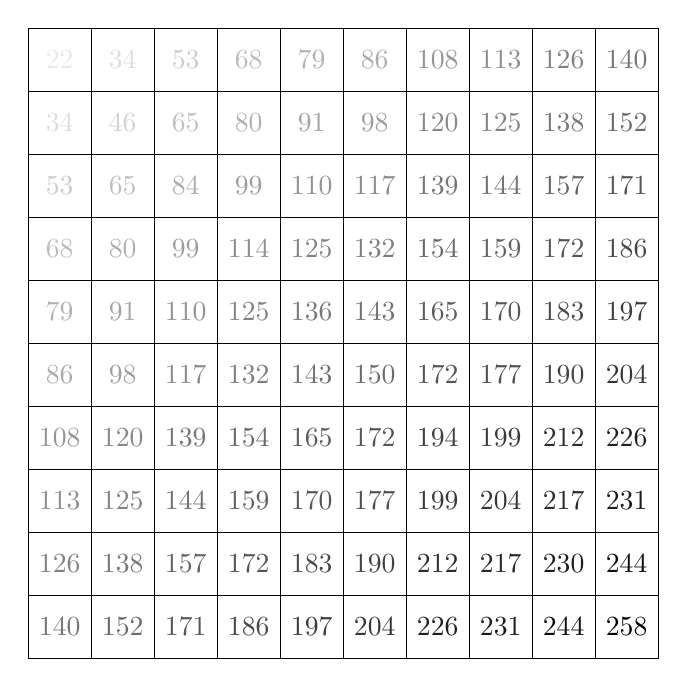
\begin{tikzpicture}[scale=0.8]
    \def\A{{11, 23, 42, 57, 68, 75, 97, 102, 115, 129}}%
    \foreach \x in {0,1,...,9} {
      \foreach \y in {0,1,...,9} {
        \draw[black] (\x, -\y) rectangle (\x+1, -\y-1);
        \pgfmathtruncatemacro\X{\A[\x]}
        \pgfmathtruncatemacro\Y{\A[\y]}
        \pgfmathtruncatemacro\result{\X+\Y}
        \pgfmathsetmacro{\C}{(\X+\Y)/(129+129)*100}
        \node[black!\C](P\x\y) at (\x+0.5, -\y-0.5) {$\result$};
      }
    }
  \end{tikzpicture}
\end{document}